\documentclass{article}
\usepackage{hyperref}
\usepackage{tikz}
\usetikzlibrary{arrows,intersections}
\usepackage{amsmath} % Required for \varPsi below

\hypersetup{
    colorlinks=true,
    linkcolor=blue,
    filecolor=magenta,      
    urlcolor=cyan,
}
\usepackage{graphicx}
\usepackage{float}
\usepackage{rotating}

\begin{document}

\title{Titanic - ML Project}
\author{Bogdanowicz Michal Kamil, Geraci Luca}

\maketitle

\begin{abstract}
Report of the project for the course of ML 2019/2020
\end{abstract}


\section{Proposition}
The proposition is using a set of machine learning methods to predict the people that would survive the Titanic sinking of 15 April 1912.

The methods that have been used are:

\begin{enumerate}  
\item Logistic Regression TODO
\item Decision trees and Random Forest
\item Neural Networks TODO
\end{enumerate}

\section{Data}
\subsection{Incomplete Data}

The Data propsed to the professor was incomplete. It heavily reduced the avialble data to perform the best practices for evaluating a model. The test and training were already separated and ground truth was missing. So the complete dataset has been taken from the internet. In addition the complete list of surviors can be found at the wikipedia page \href{https://en.wikipedia.org/wiki/Passengers_of_the_RMS_Titanic}{here} (not a ML-friendly format).
This data sadly is used to cheat on the kaggle competition. Making it a quite infamous one.

\subsection{Data Format}

\begin{itemize}
\item Ticket class
\item Survival 
\item Name
\item Sex
\item Age in years
\item sibsp : number of siblings / spouses aboard the Titanic <-- This might be problematic as it doesn't seem to make much sense.
\item parch : number of parents / children aboard the Titanic<-- This might be problematic as it doesn't seem to make much sense.
\item Ticket number	
\item Fare
\item Cabin/s assigned
\item Port of Embarkation	
\item Rescue Boat
\item Body
\item Destination
\end{itemize}

With additional notes of :
Ticket class: A proxy for socio-economic status (SES)
1st = Upper
2nd = Middle
3rd = Lower

age: Age is fractional if less than 1. If the age is estimated, is it in the form of xx.5

sibsp: The dataset defines family relations in this way
Sibling = brother, sister, stepbrother, stepsister
Spouse = husband, wife (mistresses and fiancés were ignored)

parch: The dataset defines family relations in this way
Parent = mother, father
Child = daughter, son, stepdaughter, stepson
Some children travelled only with a nanny, therefore parch=0 for them.



\subsection{Data Preparation}
The data cannot be used as it is.
The names are going to be deleted, as that should not inlfuence the resut.

\section{Logistic Regression}
One important remark. Since a lot of the data is a binary variable (0,1). The square of 0 and 1 comes back to the same value. That means that eleveting features which have only values 0 and 1 adds nothing to the model. Even more, it adds a fully correlated feature. Which has a negative impact on the model (even though it has not been the case empirically for this model. The reasons seems to be that the ensuring overestimation has no effect on the final result. The reasoning used still stands : Avoid correlated features for ML).
\\
This is the procedure that has been used to select the model.

\begin{enumerate}  
\item Choose the maximum polynomial to use by comparing the measures with CV (Cross Validation)

\item Check for Bias and variance by visualizing the Error in CV and Error on Training set on a graph with X as the degree of polynomial
\item Choose the regularization parameter that reducces the CV Error the most by using the polynomial choseon and Lambda going from 0.01 to 5.
\end{enumerate}
\begin{tikzpicture}[y=10cm, x=2.5cm]

% horizontal axis
\draw[->] (1,0) -- (5,0) node[anchor=north] {};
% labels
\draw	(1,0) node[anchor=north] {1}
		(2,0) node[anchor=north] {2}
		(3,0) node[anchor=north] {3}
		(4,0) node[anchor=north] {4}
		(5,0) node[anchor=north] {5};

\draw	(1,0.1) node[anchor=east] {0.1}
		(1,0.2) node[anchor=east] {0.2}
		(1,0.3) node[anchor=east] {0.3}
		(1,0.4) node[anchor=east] {0.4}
		(1,0.5) node[anchor=east] {0.5}
		(1,0.6) node[anchor=east] {0.6};

% vertical axis
\draw[->] (1,0) -- (1,0.7) node[anchor=east] {MAE};

% Error Training
\draw (1,0.18352) -- (2,0.18029) -- (3,0.27298)  -- (4,0.33461) -- (5, 0.58153);
\draw (1.5,0.3) node {$J(\theta )_{cv}$}; %label

% Error CV
\draw (1,0.19481) -- (2,0.19101) -- (3,0.27659)  -- (4,0.33535) -- (5, 0.57908);
\draw (1.7,0.075) node {$J(\theta )_t$}; %label

\end{tikzpicture}


\section{Decision trees and random forest}
\subsection{Introduction to decision trees}
A decision tree builds upon iteratively asking questions to partition data.
Our aim is to increase the predictiveness of the model as much as possible at each partitioning so that the model keeps gaining information about the dataset.
There are two ways to measure the quality of a split:
\begin{enumerate}
	\item Gini-Index: The measure is about the impurity of a node. The aim is to reduce the impurity (reduce randomness) of data to achieve correct classification (labeling).
	\item Information Gain (Entropy):
	The information gain is the difference between entropy before and after the split.
	When splitting decision trees try to be more predictive, less impure and reduce entropy. Entropy is a measure of uncertainty or randomness. The more randomness a variable (feature) has, the higher the entropy is.  
\end{enumerate}

\subsection{Introduction to random forests}
Random forest is an ensemble of many decision trees. Random forests are built using a method called bagging in which each decision tree is used as parallel estimator.
Random forests reduce the risk of overfitting and accuracy is much higher than a single decision tree. Furthermore, decision trees in a random forest run in parallel so that the time does not become a bottleneck.


\subsection{Procedure}
We used the M5PrimeLab Octave toolbox as follows:
\begin{enumerate}  
	\item Normalize data introducing Dummy Variables and transform feature in numerical data
	\item Build and plot the decision tree to inspect generated number of rules
	\item Use 10-fold Cross Validation to calculate the key indicators MAE, MSE, RMSE, RRMSE, R2, nRules, nVars
	\item Build and plot the precision tree to inspect generated number of rules
	\item Use 10-fold Cross Validation on precision tree to calculate the key indicators MAE, MSE, RMSE, RRMSE, R2, nRules, nVars
	\item Calculate prediction, training set mean and input variable contributions
	\item Extract the decision rules from the tree
	\item Build tree forest (ensemble) 
	\item Calculate the out-of-bag Mean Squared Error (MSE) 
	\item Plot the variable importance
	\item Predict the forest
	\item Use 10-fold Cross Validation to evaluate the predictive performance of the forest
\end{enumerate}

\subsection{Results}

\newpage
\vfill
\begin{sidewaysfigure}[h]
	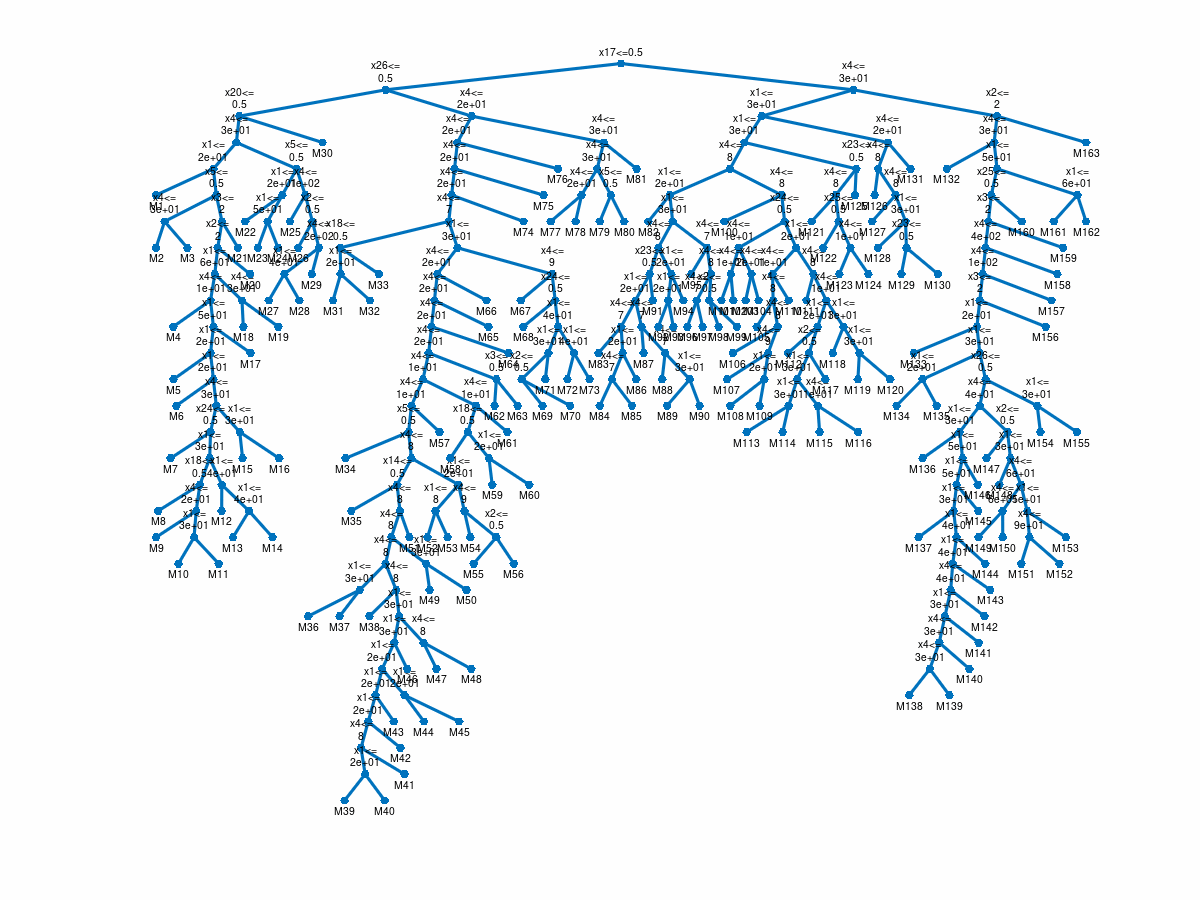
\includegraphics[width=\textwidth,height=\textheight,keepaspectratio]{decision_tree.png}
	\caption{decision tree}
\end{sidewaysfigure}	
\begin{sidewaysfigure}[h]
	\centering
	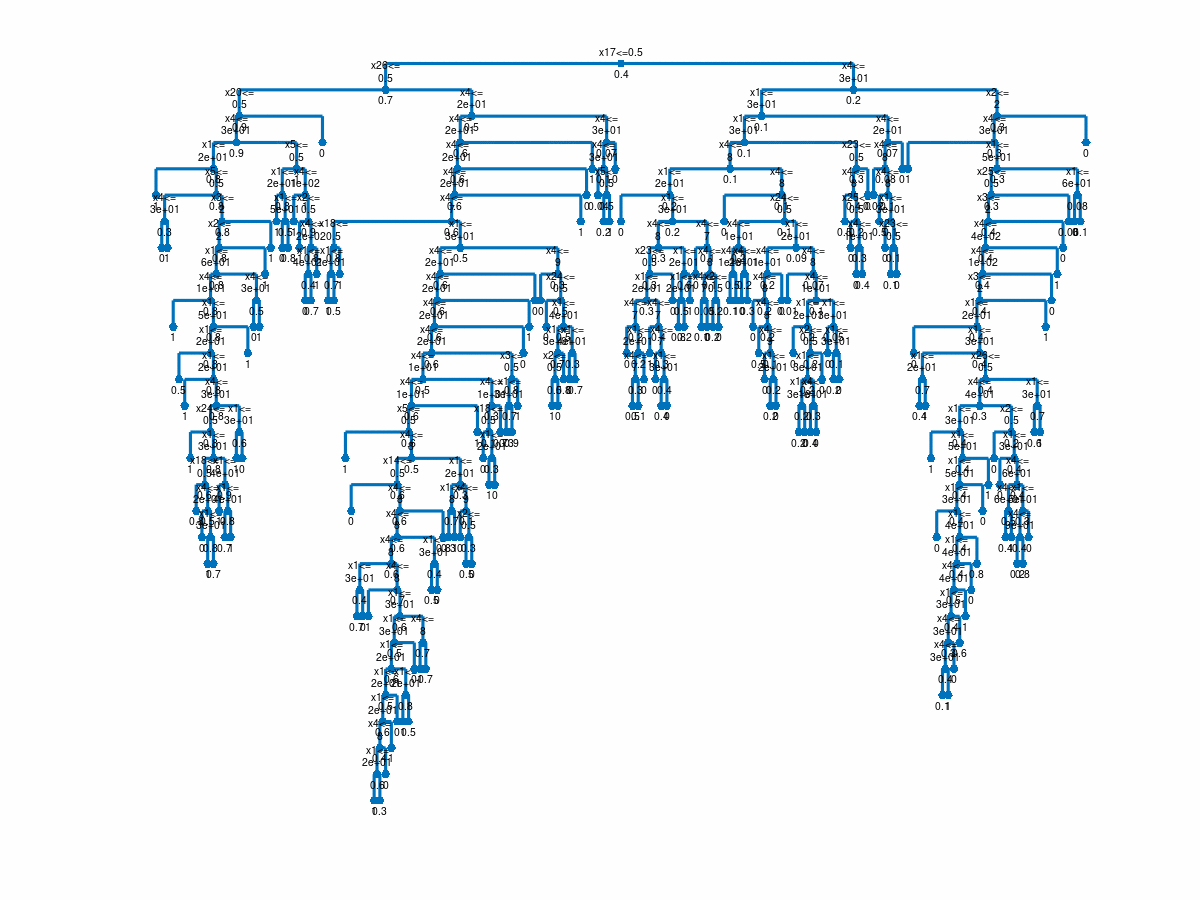
\includegraphics[width=\textwidth,height=\textheight,keepaspectratio]{precision_tree.png}
	\caption{precision tree}
\end{sidewaysfigure}
\vfill
\clearpage


	
\subsection{Lesson learned}
\subsubsection{Advantages of Decision Trees}
\begin{enumerate}
	\item No normalization or scaling of features
	\item Suitable for mixed feature data types
	\item Easy results interpretation
\end{enumerate}

\subsubsection{Disadvantages of Random Trees}
\begin{enumerate}
\item Prone to overfit and need to build forests to get good results
\end{enumerate}

\subsubsection{Advantages of Random Forests}
\begin{enumerate}
	\item Powerful, highly accurate model on many different problems
	\item No normalization or scaling of features
	\item Suitable for mixed feature data types
	\item Parallel computation for stable performance
\end{enumerate}

\subsubsection{Disadvantages of Random Forests}
\begin{enumerate}
	\item Not a good choice for high-dimensional data
\end{enumerate}


\section{Conclusion}
Write your conclusion here.

\end{document}
